\documentclass[11pt]{article}
\usepackage[utf8]{inputenc}
\usepackage[T1]{fontenc}
\usepackage[English]{babel}
\usepackage[a4paper, portrait, margin=2.5cm]{geometry}
\geometry{verbose,tmargin=2.2cm,bmargin=1.9cm,lmargin=1.8cm,rmargin=1.8cm}
\renewcommand{\baselinestretch}{1.5}
\usepackage[font={footnotesize,it}]{footnote}
\usepackage{setspace}
\usepackage[toc,page]{appendix}
\bibliographystyle{apalike}
\usepackage{fancyhdr}
\usepackage{lastpage}
\usepackage{xcolor}
\usepackage{bbm}
\usepackage{mathtools,amssymb}
\usepackage{caption}
\usepackage{subcaption}
\usepackage{booktabs, caption}
\usepackage[labelfont=bf]{caption}
\usepackage[margin = 0.5cm]{caption}
\usepackage[figurename=Figure]{caption}
\usepackage{subcaption}
\captionsetup[table]{labelsep=colon,labelfont={bf,it},textfont=it}
\captionsetup[figure]{labelsep=colon,justification=raggedright,labelfont={bf,it},textfont=it}
\usepackage{longtable}
\usepackage{adjustbox}
\usepackage{multirow}
\usepackage{graphicx}
\usepackage{wrapfig}
\usepackage{float}
\usepackage[final]{pdfpages}
\usepackage{import}
\usepackage{subfiles}
\usepackage{amsmath}
\usepackage{bbm}
\usepackage{lipsum}
\usepackage{rotating}
\usepackage[round]{natbib}   % omit 'round' option if you prefer square brackets
\usepackage[linktoc=all]{hyperref}
\hypersetup{hidelinks}
\usepackage{enumitem}
\setlength{\parindent}{2em}
\usepackage{url}
\usepackage{verbatim}
\usepackage{titlesec}
\renewcommand{\arraystretch}{0.75}
\usepackage{threeparttable}

\pagestyle{fancy}
\fancyhf{}
\rhead{Astrid Fugleholm, Jacob Strabo, \& Jørgen Høst}
\lhead{Advanced Microeconometrics}
\fancyfoot[C]{Page \thepage\ of \pageref{LastPage}}

\renewcommand{\headrulewidth}{0.4pt}
\renewcommand{\footrulewidth}{0.4pt}

\renewcommand{\tablenotes}{\setlength\labelsep{0pt}}
\renewcommand{\tablenotes}{\vspace{-.5em}}

\title{AME Project 1: Linear Panel Data and Production Technology}
\author{asfugleholm}
\date{September 2022}

\begin{document}

% Changing font of section titles
\titleformat{\section}
  {\normalfont\Large\scshape}{\thesection}{1em}{}
\titleformat{\subsection}
  {\normalfont\large\scshape}{\thesubsection}{1em}{}
\titleformat{\subsubsection}
  {\normalfont\normalsize\scshape}{\thesubsubsection}{1em}{}

\subfile{Title}

\section{Introduction}
Even for the uninitiated, the notion of returns to scale is fairly intuitive. Yet, the relationship between firm size and economic performance remains an empirical puzzle. Is economic performance independent of firm size? That is, does firm output proportionally follow input? If not, do bigger firms have an economic advantage or disadvantage? In this paper, we investigate whether sales rates depend on firm size using data from French manufacturing firms between 1967 and 1978. 

To do this, we run a series of regressions using three conventional linear estimators - pooled OLS, fixed effect (FE) and first differences (FD). We find no evidence of constant returns to scale for French manufacturing firms between 1967-1978. If anything, we find decreasing returns to scale. This is similar \cite{szpiro1994returns}, who in large part reject the notion of constant returns to scale in the French manufacturing industry in a model that allows for variations in returns to scale depending on company size. 

Crucially, however, we argue that these estimators are ill-suited for inference in this context and call for further work. Pooled OLS is a particularly poor estimator, as consistent POLS-estimates requires no correlation between time-invariant heterogeneity and the regressors. While FD and FE does account for this, they require a stronger assumption of (strict) exogeneity. As is by construction and illustrated by leading a variable, this assumption fails to hold. Instead, for future work, we propose to use the Arellano-Bond estimator that can potentially alleviate this issue.

\section{Data}
We use panel data for French manufacturing firms covering $N=441$ firms observed $T=12$ years during the period 1967-1978. The data contains observations on the firms' deflated sales, number of employees, and adjusted capital stock. Output is measured as the log of deflated sales, labor as the log of employment, and capital as the log of adjusted capital stock. All variables are time-demeaned implying that any effect specific to calendar time are discarded. The binned scatterplot in Figure \ref{fig:fig_bin_plot} shows a particularly striking linear relationship between economic performance (log sales) and firm size. This lends itself to investigate whether it is in fact the case that economic performance is independent of firm size or, equivalently, that we have constant returns to scale. 

\begin{figure}[H]
    \centering
    \caption{The link between firm size and economic performance}
    \label{fig:fig_bin_plot}
    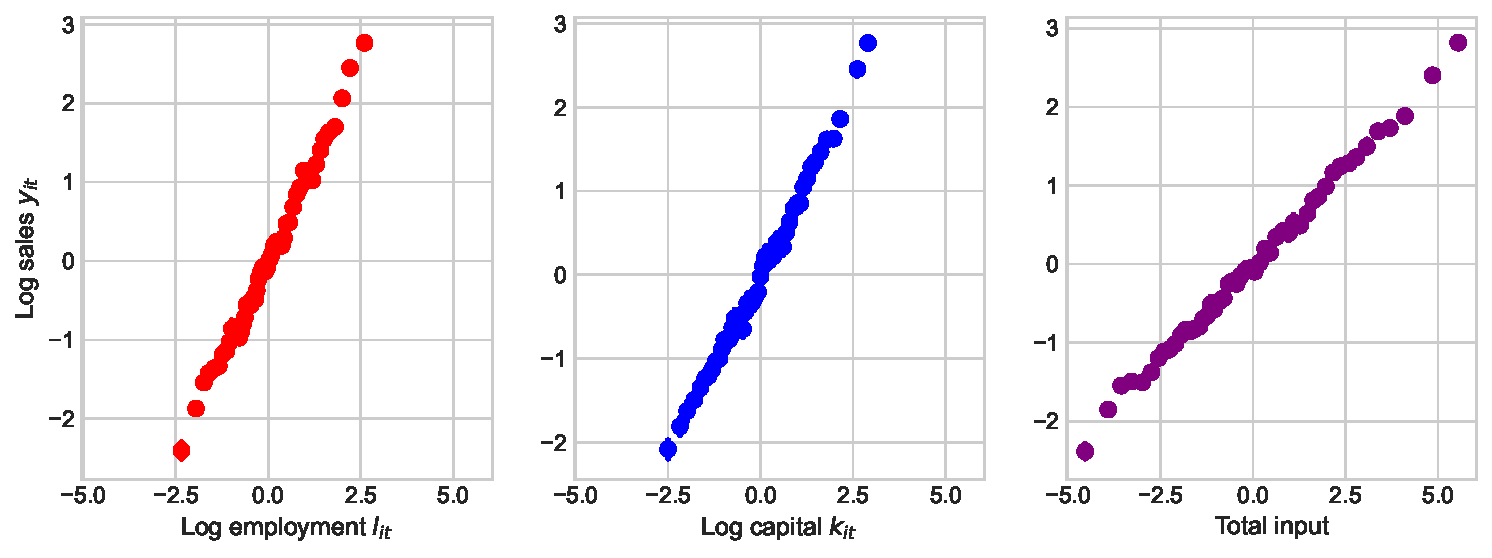
\includegraphics[scale=0.7]{fig1.pdf}
    \caption*{Note: Scatter plot with 50 equally sized bins of log capital and log employment.}
\end{figure}

\section{Cobb-Douglas Producton Function}
As in standard economic theory, we assume that firms produce according to a Cobb-Douglas production function
\begin{equation}
    Y = F(K,L) = AK^{\beta_K}L^{\beta_L}, 
\end{equation}
where $Y$ is output generated by total factor productivity (TFP) $A>0$, capital $K$, and labor $L$. Output elasticities of capital and labor are denoted $\beta_K$ and $\beta_L$, resp. Capital and labor are observed, while TFP is unobserved. Expressing the model in compliance with our data gives the following relationship: 
\begin{equation}
\label{LinearModel}
    y_{it} = \beta_K k_{it} + \beta_L l_{it} + \eta_{it}, 
\end{equation}
where $y_{it}$, $k_{it}$, $l_{it}$, and $\nu_{it}$ are the log of deflated sales, adjusted capital stock, employment, and TFP, resp., in firm $i$ at time $t$. 

Economic theory typically assumes that firms have constant returns to scale in their production; changing all inputs by the same factor leads to a proportional change in output in which case, the production function satisfies   
\begin{equation}
    F(\lambda K,\lambda L)=\lambda F(K,L),
\end{equation}
where $\lambda \geq 0$. 
However, firms' production may alternatively exhibit increasing or decreasing returns to scale with output changing more or less, resp., than proportionately to changes in inputs. Our empirical analysis aims at testing the validity of the assumption of constant returns to scale.

\section{Econometric Model}
We consider the following linear unobserved effects model: 
\begin{equation}
\label{UELinearModel}
    y_{it} = \beta_K k_{it} + \beta_L l_{it} + c_i + u_{it}, 
\end{equation}
where $y_{it}$, $k_{it}$, and $l_{it}$, are the log of deflated sales, adjusted capital stock, and employment, resp.; $c_i$ are firm-specific time-invariant factors; and $u_{it}$ is the idiosyncratic error capturing all other time-varying factors affecting firms' production. 
In (\ref{LinearModel}), $\nu_{it}$ captures both the time-invariant and time-varying unobserved productivity factors which in model (\ref{UELinearModel}) are captured by $c_i$ and $u_{it}$, resp. Time-invariant factors in $c_i$ could be the location of a factory which may or may not be geographically favorable to a particular firm, for instance with ease of access to coal. Time-varying factors in $u_{it}$ could be supply chain shocks or labor strikes affecting the price and quantity of production inputs.

Our parameters of interest are $\beta_K$ and $\beta_L$, capturing the returns to scale, with $\beta_K+\beta_L > 1$ implying increasing, $\beta_K+\beta_L<1$ implying decreasing, and $\beta_K+\beta_L=1$ implying constant returns to scale. Testing the assumption of constant returns to scale thus amounts to the null and alternative hypotheses 
\begin{equation}
    \mathcal{H}_0: \beta_K+\beta_L=1 \quad \text{and} \quad \mathcal{H}_A: \beta_K+\beta_L\ne1.
\end{equation}
Throughout the paper, we employ the following notation: $K=2$ is the number of regressors in our model; $T=12$ is the number of time periods in our data; $N=441$ is the number of cross sectional units in our data; $\textbf{x}_{it}=\{k_{it},l_{it}\}$ is a $(1\times2)$ vector of regressors; and $\beta=\{\beta_K,\beta_L\}$ is a $(1\times2)$ vector of parameters. 

\subsection{The Ordinary Least Squares (OLS) Estimator}
A natural starting point is to examine the relationship between production in- and output by estimating the linear model in (\ref{UELinearModel}) using Ordinary Least Squares (OLS). As the time-specific means have all ready been subtracted in our data, our OLS analysis, is in fact a time fixed effects model.

OLS is consistent, i.e. converges in probability to the true parameter (\cite{AP}), if two assumptions hold, cf. \cite{Wooldrige_2010_4}: 
\begin{itemize}
    \item[] \textbf{OLS.1}: $\mathbb{E}[\textbf{x}_{it}u_{it}]=0 \quad \forall i\in N, \quad \forall t \in T$, i.e. regressors are uncorrelated with the idiosyncratic error. 
    \item[] \textbf{OLS.2}: $\text{Rank}\left[\mathbb{E}[\textbf{X}_i'\textbf{X}_i]\right]=K\quad \forall i\in N$, i.e. the matrix of regressors has full rank. 
\end{itemize}
OLS is efficient, i.e. has a small asymptotic variance (\cite{Wooldridge_2016_5}), if an additional assumption holds, cf. \cite{Wooldrige_2010_4}:
\begin{itemize}
    \item[] \textbf{OLS.3}:  $\mathbb{E}[u^2\textbf{X}_i'\textbf{X}_i]=\sigma^2\mathbb{E}[\textbf{X}_i'\textbf{X}_i] \quad \forall i\in N$ where $\sigma^2\equiv \mathbb{E}[u^2]$, i.e. the idiosyncratic errors are homoskedastic and thus have constant variance. 
\end{itemize}
In our setting, OLS is consistent if capital, labor, and firm-specific effects are unaffected by omitted variables observed in the same time period, and capital and labor do not exhibit a linear relationship. OLS is efficient if capital and labor explain (most of) the variation in output across firms. 
As firm-specific fixed effects are unobserved, $c_i$ is effectively included in a composite error term $\eta_{it}=c_i+u_{it}$. Hence, OLS.1 implies that capital and labor are uncorrelated with both the idiosyncratic error as well as firm-specific fixed effects: $\mathbb{E}\left[u_{it}|\textbf{x}_{it},c_i\right]=0$. Since more productive firms likely employ different levels of capital and labor than less productive firms, OLS.1 is unlikely to hold, and OLS will thus be inconsistent. Seeing that the random effects (RE) estimator also relies on firm-specific fixed effects being orthogonal to the regressors, it is also assumed to be inconsistent. Therefore, we turn to the first differences (FD) and fixed effects (FE) estimators with different approaches to removing firm-specific fixed effects. 

\subsection{The Fixed Effects (FE) Estimator}
The FE estimator removes firm-specific fixed effects by subtracting from each variable its mean: 
\begin{equation*}
    y_{it}-\Bar{y}_i=\beta_K(k_{it}-\Bar{k}_i)+\beta_L(l_{it}-\Bar{l}_i)+c_i-\Bar{c}_i+u_{it}-\Bar{u}_i \Leftrightarrow
\end{equation*}
\begin{equation}
\label{FE_model}
    \ddot{y}_it = \beta_K\ddot{k}_{it}+\beta_L\ddot{l}_{it}+\ddot{u}_{it}, \quad t=1,...,T, 
\end{equation}
where $c_i$ vanishes as it is constant over time. 
% \begin{equation}
% \label{FE_hetero_variance}
%     \widehat{Avar}(\widehat{\beta}_{FD}) = (\ddot{\textbf{X}}'\ddot{\textbf{X}})^{-1} \left(\sum_{i=1}^N\ddot{\textbf{X}}_i'\hat{\ddot{\textbf{u}}}_i\hat{\ddot{\textbf{u}}}_i'\ddot{\textbf{X}}_i\right)(\ddot{\textbf{X}}'\ddot{\textbf{X}})^{-1}.
% \end{equation}
FE consistently estimates $\beta$ as $N\rightarrow\infty$ for fixed T under FE.1 and FE.2, cf. \cite{Wooldrige_2010_10}:
\begin{itemize}
    \item[] \textbf{FE.1}: $\mathbb{E}[\Ddot{\textbf{x}}_{it}\Ddot{u}_{is}]=0 \quad \forall i\in N \quad \text{and} \quad s,t \in T$, i.e. the idiosyncratic errors are strictly exogeneous meaning that they are uncorrelated with the regressors in period $t$ and all other periods. 
    \item[] \textbf{FE.2}: $\text{Rank}\left[\mathbb{E}\left[\Ddot{\textbf{X}_i}'\ddot{\textbf{X}_i}\right]\right] \quad \forall i\in N$, i.e. the matrix of regressors $\Ddot{\textbf{X}_i}$ has full rank meaning that the matrix product $\Ddot{\textbf{X}}'\ddot{\textbf{X}_i}$ is invertable. This assumption rules out the presence of time-invariant regressors in our model. 
\end{itemize}
FE is asymptotically efficient under FE.3, cf. \cite{Wooldrige_2010_10}:
\begin{itemize}
    \item[] \textbf{FE.3}: $\mathbb{E}\left[\textbf{u}_i\textbf{u}_i'|x_{it} c_i \right]=\sigma_u^2 \textbf{I}_T \quad \forall i \in N$, i.e. the time-demeaned idiosyncratic errors are homoskedastic and thus have constant variance.  
\end{itemize}
In our setting, FE is consistent if capital and labor are unaffected by omitted variables observed in any other time period, and capital and labor are time-variant. FE is efficient if time-demeaned capital and labor explain (most of) the variation in time-demeaned output across firms.  

Following derivations in \cite{Wooldrige_2010_10}, we define the estimator as
\begin{equation}
    \widehat{\beta}_{FE}=(\ddot{\textbf{X}}'\ddot{\textbf{X}})^{-1}\ddot{\textbf{X}}'\ddot{\textbf{y}}
\end{equation}
and its variance-covariance estimator under FE.3 as
\begin{equation}
    \widehat{Avar}(\widehat{\beta}_{FD}) = \hat{\sigma}_u^2\left(\ddot{\textbf{X}}'\ddot{\textbf{X}}\right)^{-1}, 
\end{equation}
where $\hat{\sigma}_u^2=\frac{\sum_{i=1}^N\sum_{t=1}^N\hat{\ddot{u}}_{it}^2}{NT-N-K}$, and $\ddot{\textbf{X}}$ and $\ddot{\textbf{y}}$ are resp. a $441*12\times 2$ matrix and $441*12\times1$ vector of stacked $\ddot{\textbf{x}}_{it}$ and $\ddot{\textbf{y}}_{it}$ from (\ref{FE_model}). 

\subsection{The First Difference (FD) Estimator}
The FD estimator removes firm-specific effects by subtracting the value from the previous period: 
\begin{equation*}
    y_{it}-y_{i,t-1} = \beta_K(k_{it}-k_{i,t-1}) + \beta_L(l_{it}-l_{i,t-1})+c_i-c_i+u_{it}-u_{i,t-1} \Leftrightarrow 
\end{equation*}
\begin{equation}
\label{FD_model}
    \Delta y_{it}=\beta_K\Delta k_{it} + \beta_L \Delta l_{it} + \Delta u_{it}, \quad t=2,...,T,
\end{equation}
where $c_i$ vanishes as it is constant over time.  
% \begin{equation}
% \label{FD_hetero_variance}
%     \widehat{Avar}(\widehat{\beta}_{FD})=\left(\sum_{i=1}^N\Delta \textbf{X}_i'\Delta \textbf{X}_i\right)^{-1}\left(\sum_{i=1}^N\Delta \textbf{X}_i'\widehat{\Delta u}_i\widehat{\Delta u}_i'\Delta \textbf{X}_i\right)\left(\sum_{i=1}^N\Delta \textbf{X}_i'\Delta \textbf{X}_i\right)^{-1}.
% \end{equation}
FD consistently estimates $\beta$ as $N\rightarrow\infty$ for fixed T under FD.1 and FD.2, cf. \cite{Wooldrige_2010_10}:
\begin{itemize}
    \item[] \textbf{FD.1}: $\mathbb{E}[\Delta x_{it}\Delta u_{is}]=0, \quad \forall i\in N \quad \text{and} \quad s,t \in T$, i.e. strict exogeneity as in FE.1. In fact, it is sufficient to assume that the idiosyncratic error is uncorrelated with the regressors in period $t-1$, $t$, and $t+1$: $\mathbb{E}[u_{it}|x_{i,t-1},x_{it},x_{i,t+1}]=0$. 
    \item[] \textbf{FD.2}: $\text{Rank}\left[E[\Delta \textbf{X}_i'\Delta \textbf{X}_i]\right]=K \quad \forall i\in N$, i.e. the matrix of regressors $\Delta\textbf{X}_i$ has full rank meaning that the matrix product $\Delta\textbf{X}_i'\Delta \textbf{X}_i$ is invertable. This assumption rules out the presence of time-invariant regressors in our model. 
\end{itemize}
FE is asymptotically efficient under FD.3, cf. \cite{Wooldrige_2010_10}:
\begin{itemize}
    \item[] \textbf{FD.3}: $\mathbb{E}[\textbf{e}_i\textbf{e}_i'|x_{it} c_i]=\sigma^2_e I_{T-1} \quad \forall i\in N$, where $\textbf{e}_i= \Delta \textbf{u}_{it}$, i.e. the differenced idiosyncratic errors are homoskedastic and thus have constant variance. 
\end{itemize}
In our setting, FD is consistent if capital and labor are unaffected by omitted variables observed in the previous, current, and future time period, and capital and labor are time-variant. FD is efficient if first-differenced capital and labor explain (most of) the variation in first-differenced output across firms. 

Following derivations in \cite{Wooldrige_2010_10}, we define the estimator as 
\begin{equation}
    \widehat{\beta}_{FD} = \left(\Delta \textbf{X}'\Delta \textbf{X}\right)^{-1}\Delta \textbf{X}'\Delta y
\end{equation}
and its variance-covariance under FD.3 as
\begin{equation}
    \widehat{Avar}(\widehat{\beta}_{FD})= \hat{\sigma}_u^2\left(\sum_{i=1}^N\Delta\textbf{X}_i'\Delta\textbf{X}\right)^{-1},
\end{equation}
where $\hat{\sigma}_u^2=\frac{1}{NT-N-K}\sum_{i=1}^N\sum_{t=1}^T\widehat{\Delta u}_{it}^2$, and $\Delta\textbf{X}$ and $\Delta\textbf{y}$ are resp. a $441*11\times2$ matrix and $441*11\times1$ vector of stacked $\Delta\textbf{x}_{it}$ and $\Delta\textbf{y}_{it}$ from (\ref{FD_model}).

\section{Results}
We proceed by estimating the three above mentioned panel data models in a static setting, and the results are reported in \textit{table \ref{tab:est_results}}. In any case, capital and labor have positive effects on output. A 1\% increase in capital and labor leads to a 0.70-0.55\% and 0.30-0.06\% increase in output, resp. 
\begin{table}[H]    
        \caption{Effects of Employment and Capital on Firms' Production}
        \centering
        \label{tab:est_results}
        \begin{threeparttable}     
            \begin{tabular}{lcccc}
            \toprule
                                & {} &       POLS &         FE &         FD \\
            \midrule
            Constant            & {} &        0.0 &          . &          . \\
                                & {} &    (0.005) &          . &          . \\
            Log employment, $\beta_L$      & {} &  0.6778*** &  0.6964*** &  0.5462*** \\
                                & {} &   (0.0101) &   (0.0144) &   (0.0177) \\
            Log capital stock, $\beta_K$   & {} &  0.3028*** &  0.1427*** &  0.0645*** \\
                                & {} &    (0.009) &   (0.0124) &   (0.0182) \\
            \midrule
            $N$                 & {} &        441 &        441 &        441 \\
            $T$                 & {} &        12  &        12  &        11  \\
            \bottomrule
            \end{tabular}
                \begin{tablenotes}
                \footnotesize \textit{Note:} Standard errors in parentheses, $p<0.05$*, $p<0.01$**, $p<0.001$***.
                \end{tablenotes}
        \end{threeparttable}
\end{table}

Comparing POLS with FE and FD estimates, the effect of capital on output is drastically reduced. With the two latter accounting for unobserved time-invariant heterogeneity $c_i$, this is not surprising; firms with an advantageous geographic location can produce more output and devote more resources to investments in capital stock creating upward bias in $\beta_K$. Hence, OLS is deemed inconistent. We thus turn to the FE and FD estimators and evaluate the validity of assumptions required for them to be consistent and efficient. 

\subsection{First Differences versus Fixed Effects}
% \textcolor{blue}{Further, it follows that $e_{it}$ must be serially uncorrelated for FD to be a consistent estimator \cite{Wooldridge_2016_serial_corr}}.
The FD and FE estimators both eliminate the omitted variable bias by taking the firm-specific fixed effects into account. The interpretation of $\beta$ within the two models is the same, only the estimation differs (\cite{Wooldrige_2010_10}). When $T=2$, the two estimators are numerically identical. When $N>2$, the choice between the two hinges on the level of serial correlation in the idiosyncratic errors. FE is more efficient if errors are serially uncorrelated; the differenced errors will in this case be correlated over time, although the errors themselves are not. This means that FD.3 is violated while FE.3 is not. Further, we loose an observation in the first time period and thereby some precision in our estimation when using FD ($T=12$ for FE, $T=11$ for FD). 
On the other hand, FD is more efficient than FE if the error term follows a random walk; the errors themselves are correlated over time, but the differenced errors are not. When the error term is serially correlated, first-differencing leaves only white noise.
To inform our choice between FE and FD, we perform a test for serial correlation by running the following regression 
\begin{equation}
    \widehat{\epsilon}_{it}= \rho\widehat{\epsilon}_{i,t-1}+u_{it},
\end{equation}
where $\widehat{\epsilon}_{it}$ are residuals from regression (???) and $\rho$ measures the degree of serial correlation. 
The results are reported in \textit{table \ref{tab:Serial_corr}}.
%Let's assume some random walk (could be that if an observation is low/high today, then it is likely also to be low/high tomorrow), then FE simply subtracts the time and firm specific means, whereas the error term of FD leaves only white noise. 
%\bigskip
%The choice between FD and FE depends on the level of serial correlation in the idiosyncratic errors. Following \cite{Wooldridge_2016_serial_corr}, if the idiosyncratic errors $u_{it}$ are uncorrelated to begin with, the differenced idiosyncratic $e_{it} \equiv u_{it}-u_{it-1}$ will be serially correlated. If that is the case, \textbf{FD.3} is violated and FD inconsistent. 

\begin{table}[H]
    \centering
    \caption{Test for serial correlation}
    \label{tab:Serial_corr}
    \begin{threeparttable}
        \begin{tabular}{lc}
        \toprule
                     & $\epsilon_{it}$ \\
        \midrule
        $\epsilon_{i,t-1}$, $\rho$    &         -0.2141*** \\
                     &           (0.0145) \\
        \midrule
        $N$          & 441  \\
        $T$          & 10 \\
        \bottomrule
        \end{tabular}
    \end{threeparttable}
\end{table}

We formulate a null and alternative hypothesis for the presence of serial correlation: $\mathcal{H}_0:\rho=0$ and $\mathcal{H}_A:\rho\ne0$. 
\textit{Table \ref{tab:Serial_corr}} shows that the t-statistic is significantly greater than the critical value on a 1\% level, so we reject $\mathcal{H}_0$ and conclude that the errors are serially correlated. This suggests that in our setting, FD is more efficient than FE and thus the preferred estimator. 

We also conduct a test for strict exogeneity required for both FD and FE to be consistent. This is done by include a lead of employment (results are analogous to including a lead of capital). 

\begin{table}[H]
    \centering
    \caption{Test for strict exogeneity}
    \label{tab:strict_exo}
    \begin{threeparttable}
        \begin{tabular}{lc}
        \toprule
                                                    & FE       \\
        \midrule
        Log employment, $\beta_L$                    &  0.556*** \\
                                                     &  (0.0226) \\
        Log capital stock, $\beta_K$                &  0.1323*** \\
                                                     &  (0.0129) \\
        Log employment +1, $\beta_L$ for $t+1$      &  0.1688*** \\
                                                 &  (0.0218) \\
                                \midrule
        $N$                                         &        441 \\
        $T$                                        &         11  \\
        \bottomrule
        \end{tabular}
            \begin{tablenotes}
                \footnotesize \textit{Note:} Standard errors in parentheses, $p<0.05$*, $p<0.01$**, $p<0.001$***.
            \end{tablenotes}
    \end{threeparttable}
\end{table}

Recall \textbf{FE.1}/\textbf{FD.1}. In the context of this paper, these imply that predetermined log sales at time $t$ cannot be correlated be with log employment in any other time period, when controlling for unobserved time-invariant heterogeneity (\cite{Wooldridge_2016_serial_corr}). The result from table \ref{tab:strict_exo} shows that this is fortunately the case. As such, we are left with inconsistent estimates from FD and FE in table \ref{tab:est_results}.

\subsection{Testing Hypothesis of Constant Returns to Scale}
For practical purposes, we elect to to test the phenomenon of constant returns to scale despite our inconsistent estimates. To do this, define define the following Wald statistics of some linear hypothesis $\mathbf{R\beta=r}$:
\begin{equation*}
    (\mathbf{R} \widehat{\boldsymbol{\beta}}-\mathbf{R} \boldsymbol{\beta})^{\prime}\left[\mathbf{R}(\mathbf{V} / N) \mathbf{R}^{\prime}\right]^{-1}(\mathbf{R} \widehat{\boldsymbol{\beta}}-\mathbf{R} \boldsymbol{\beta}) \stackrel{d}{\approx} \chi_Q^2
\end{equation*}

In the context of this paper, $\mathbf{R}=\left[
    \begin{array}{ll}
    1 & 1 
    \end{array}\right]$ with $\mathbf{r=1}$. 

For the $FD$- and $FE$-model, we find a test statistics of $\chi^2 (1)=122,656$  and $\chi^2 (1)=74,256$, respectively, with $\mathbf{Q}=rank(\mathbf{R})=1$ degrees of freedom. These test statistics are way above the critical value with p-value equal to zero. On the basis of this test, we therefore reject the notion of constant of returns to scale. However, as established before, we emphasize the questionable validity of this test as the strict exogeneity assumption is violated.

\section{Discussion}
As evidenced above, we are left dissatisfied with our estimates from Table \ref{tab:est_results}. First, we are unwilling to assume that labor and capital input is uncorrelated with unobserved time-invariant heterogeneity $c_i$. We gave an example of geographic advantage for specific French manufacturing which renders POLS an inconsistent estimator. We then turn to examining the link between firm size and economic performance using $FE$ and $FD$. Despite accounting for the time-invariant heterogeneity, the assumption of strict exogeneity is violated which renders $FD$ and $FE$ inconsistent estimators. 

To account for this crucial problem, we can turn to employ dynamic panel methods, one example being the Arellano-Bond estimator. In short, this is consistent under the assumption of sequential exogeneity. That is, any \textit{previous} realisations of, say, log employment, is uncorrelated with \textit{current} log sales.

If we assume a panel data model on the form $y_{i t}=\rho y_{i t-1}+\mathbf{x}_{i t}\beta+c_{i}+\,u_{i t}$. By taking first differencing, $\Delta y_{t t}=\rho\Delta y_{t t-1}+\Delta{\bf x}_{t t}^{\prime}\beta+\Delta u_{t t}$. The idea here is using log sales from two years prior as instruments ($z_{it}=y_{t-2}$) for the difference in previous log sales ($\Delta y_{t-1}$). To see why, consider that instruments must be:

\begin{enumerate}
    \item Exogenous: $E\left[\mathbf{z}_{i t} u_{i t}\right]=E\left[y_{t-2}\Delta u_{it}\right]=E\left[y_{t-2} (u_{t}-u_{i t-1})\right]=0$
    \item Relevant: $E\left[y_{t-2}\Delta y_{t-1}\right]=E\left[y_{t-2}(y_{t-1}-y_{t-2})\right]\neq 0$
\end{enumerate}

To sum up, any random labor strike or supply chain disruptions at time $t$ which lives in the idiosyncratic error term $u_{it}$ had no influence on log sales two years prior. On the other hand, log sales two years prior are naturally correlated with the difference in log sales one and two years prior.

\section{Conclusion}
In this paper, we examine the link between firm size and performance. We find no evidence of constant returns to scale - that is firm output proportionally follows input. In fact, our results suggest decreasing returns to scale, implying that bigger is not always better. 

However, we argue that estimating the relationship between firm size and economic performance by pooled $OLS$, $FD$ or $FE$ is not ideal. Unobserved time-invariant heterogeneity, such as geographic advantages specific to certain firms, renders $POLS$ a particularly poor estimator. While this is accounted for in a $FD$ and $FE$-estimation, the assumption of strict exogeneity nedded for consistency is by construction violated. Instead, we propose to use the Arellano-Bond estimator which log sales two or more years prior as instrument(s). This is likely to alleviate the issue of inconsistent estimates. 


\newgeometry{verbose,tmargin=1.9cm,bmargin=1.7cm,lmargin=1.5cm,rmargin=1.5cm}
%Resetting the numbering as we are now in references/appendix:

\newpage
\begin{small}
\bibliography{References.bib}
\end{small}

%TC:newcounter -char

\end{document}

% Forskellen på FD og FE er, at i FD må der gerne være faktorer i fejlleddet fra periode t-2 og bagud, som påvirker X i periode t - men i FE må der ikke være faktorer i fejlleddet fra nogen som helst periode bagud i tid (og foran i tid for den sags skyld), som påvirker X i periode t. Derfor må forskellen på resultaterne fra de to estimatorer komme fra det faktum, at FD tager effekterne fra fejlleddet med fra bagud i tid, hvilket FE ikke gør, og derfor er beta'erne fra FE højere end beta'erne fra FD. 

% Da der både er indeholdt tidsvarierende og tidsinvariante faktorer i TFP (A), som ikke er observeret, så må vi forvente, at selvom vi korrigere for firm fixed effects ved at bruge enten FE eller FD, så vil der stadig være nogle tidsvarierende faktorer i fejlleddet, som påvirker productiviteten og dermed giver bias i vores estimater. Så det kan vi også diskutere i resultatafsnittet. 

% From Wooldridge (2016, chapter 14 on Advanced Panel Data Methods, p. 434-460):

% It is a good thing if FD and FE produce roughly the same results -> they do not in our case which suggests that there is some issue with at least one of them in that some of the assumptions are violated. 

% Cannot test for serial correlation in the pure errors - only in the time-demeaned and the differenced. If there is no serial correlation in the differenced errors, then FD is better than FE. If there is serial correlation in the differenced errors, then FE is better than FD. 

% Inference for FE is sensitive to violations of the assumptions if N is small and T is large. The problem is not as big when using FD. 

% If the strict exogeneity assumption is violated (for example if a lagged dependent variable is included among the regressors or there is feedback between u and future outcomes of the regressors) then FE is substantially less biased than FD. The bias in the FD does not depend on T, while that for the FE estimator tends to zero at the rate 1/T, so it gets smaller the greater T is. See Wooldridge (2010) chapter 10.7. 

% From Wooldridge (2016, p. 440 in chapter 14 on Advanced Panel Data Methods): "Generally, it is difficult to choose between FE and FD when they give substantively different results. It makes sense to report both sets of results and tro try determine why they differ."